\documentclass{beamer}
\usetheme{metropolis}
\title{LEGO Mindstorms Line Following Project}
\author{Aniruddha Pal, Markus Wiktorin}
\date{23rd of September 2016}
\institute{University of Applied Science, Bonn-Rhein-Sieg}
\begin{document}
	\maketitle
	\begin{frame}
		\frametitle{Task}
		Program a LEGO robot which can follow a line.
		
		Light conditions and track can change, the robot should work under different conditions.
	\end{frame}
	\begin{frame}
		\frametitle{Approaches}
		\begin{enumerate}
			\item One light sensor in front of the robot
			\item Two light sensors in front of the robot
			\item Two light sensors in front of the robot using PID
			\item Two light sensors, ultrasonic sensor and touch sensor in front of the robot using PID
		\end{enumerate}
	\end{frame}
	\begin{frame}
		\frametitle{1. Approach (one light sensor)}
		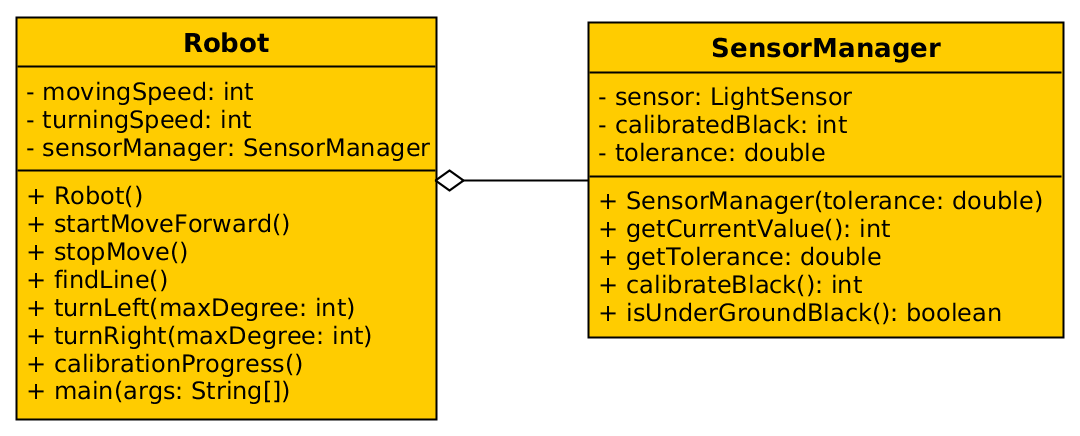
\includegraphics[width=\textwidth, height=\textheight, keepaspectratio]{firstApproach.png}
		\\
		Light sensor tries to stay in the middle of the line. If it looses the line it looks left and right in order to find it again.
		\\
		Bad approach but we tried to use object oriented concepts.
	\end{frame}
	\begin{frame}
		\frametitle{2. Approach (two light sensors)}
		
	\end{frame}
	\begin{frame}
		\frametitle{3. Approach (two light sensors + PID)}
		
	\end{frame}
	\begin{frame}
		\frametitle{4. Approach (two light, ultrasonic, touch sensor + PID)}
		\begin{itemize}
			\item We found some working values for PID in the third approach
			\item The robot is also fast on straights
			\item Next improvement: Make it possible to go on the same track with other robots
			\begin{itemize}
				\item Use ultrasonic in the front in order to detect other robots
				\item This was not working realiable, thats why we added the touch sensor
				\item The robot can still crash when it goes to turns, but on straights it is working good
			\end{itemize}
		\end{itemize}
	\end{frame}
	\begin{frame}
		\frametitle{Our robot}
		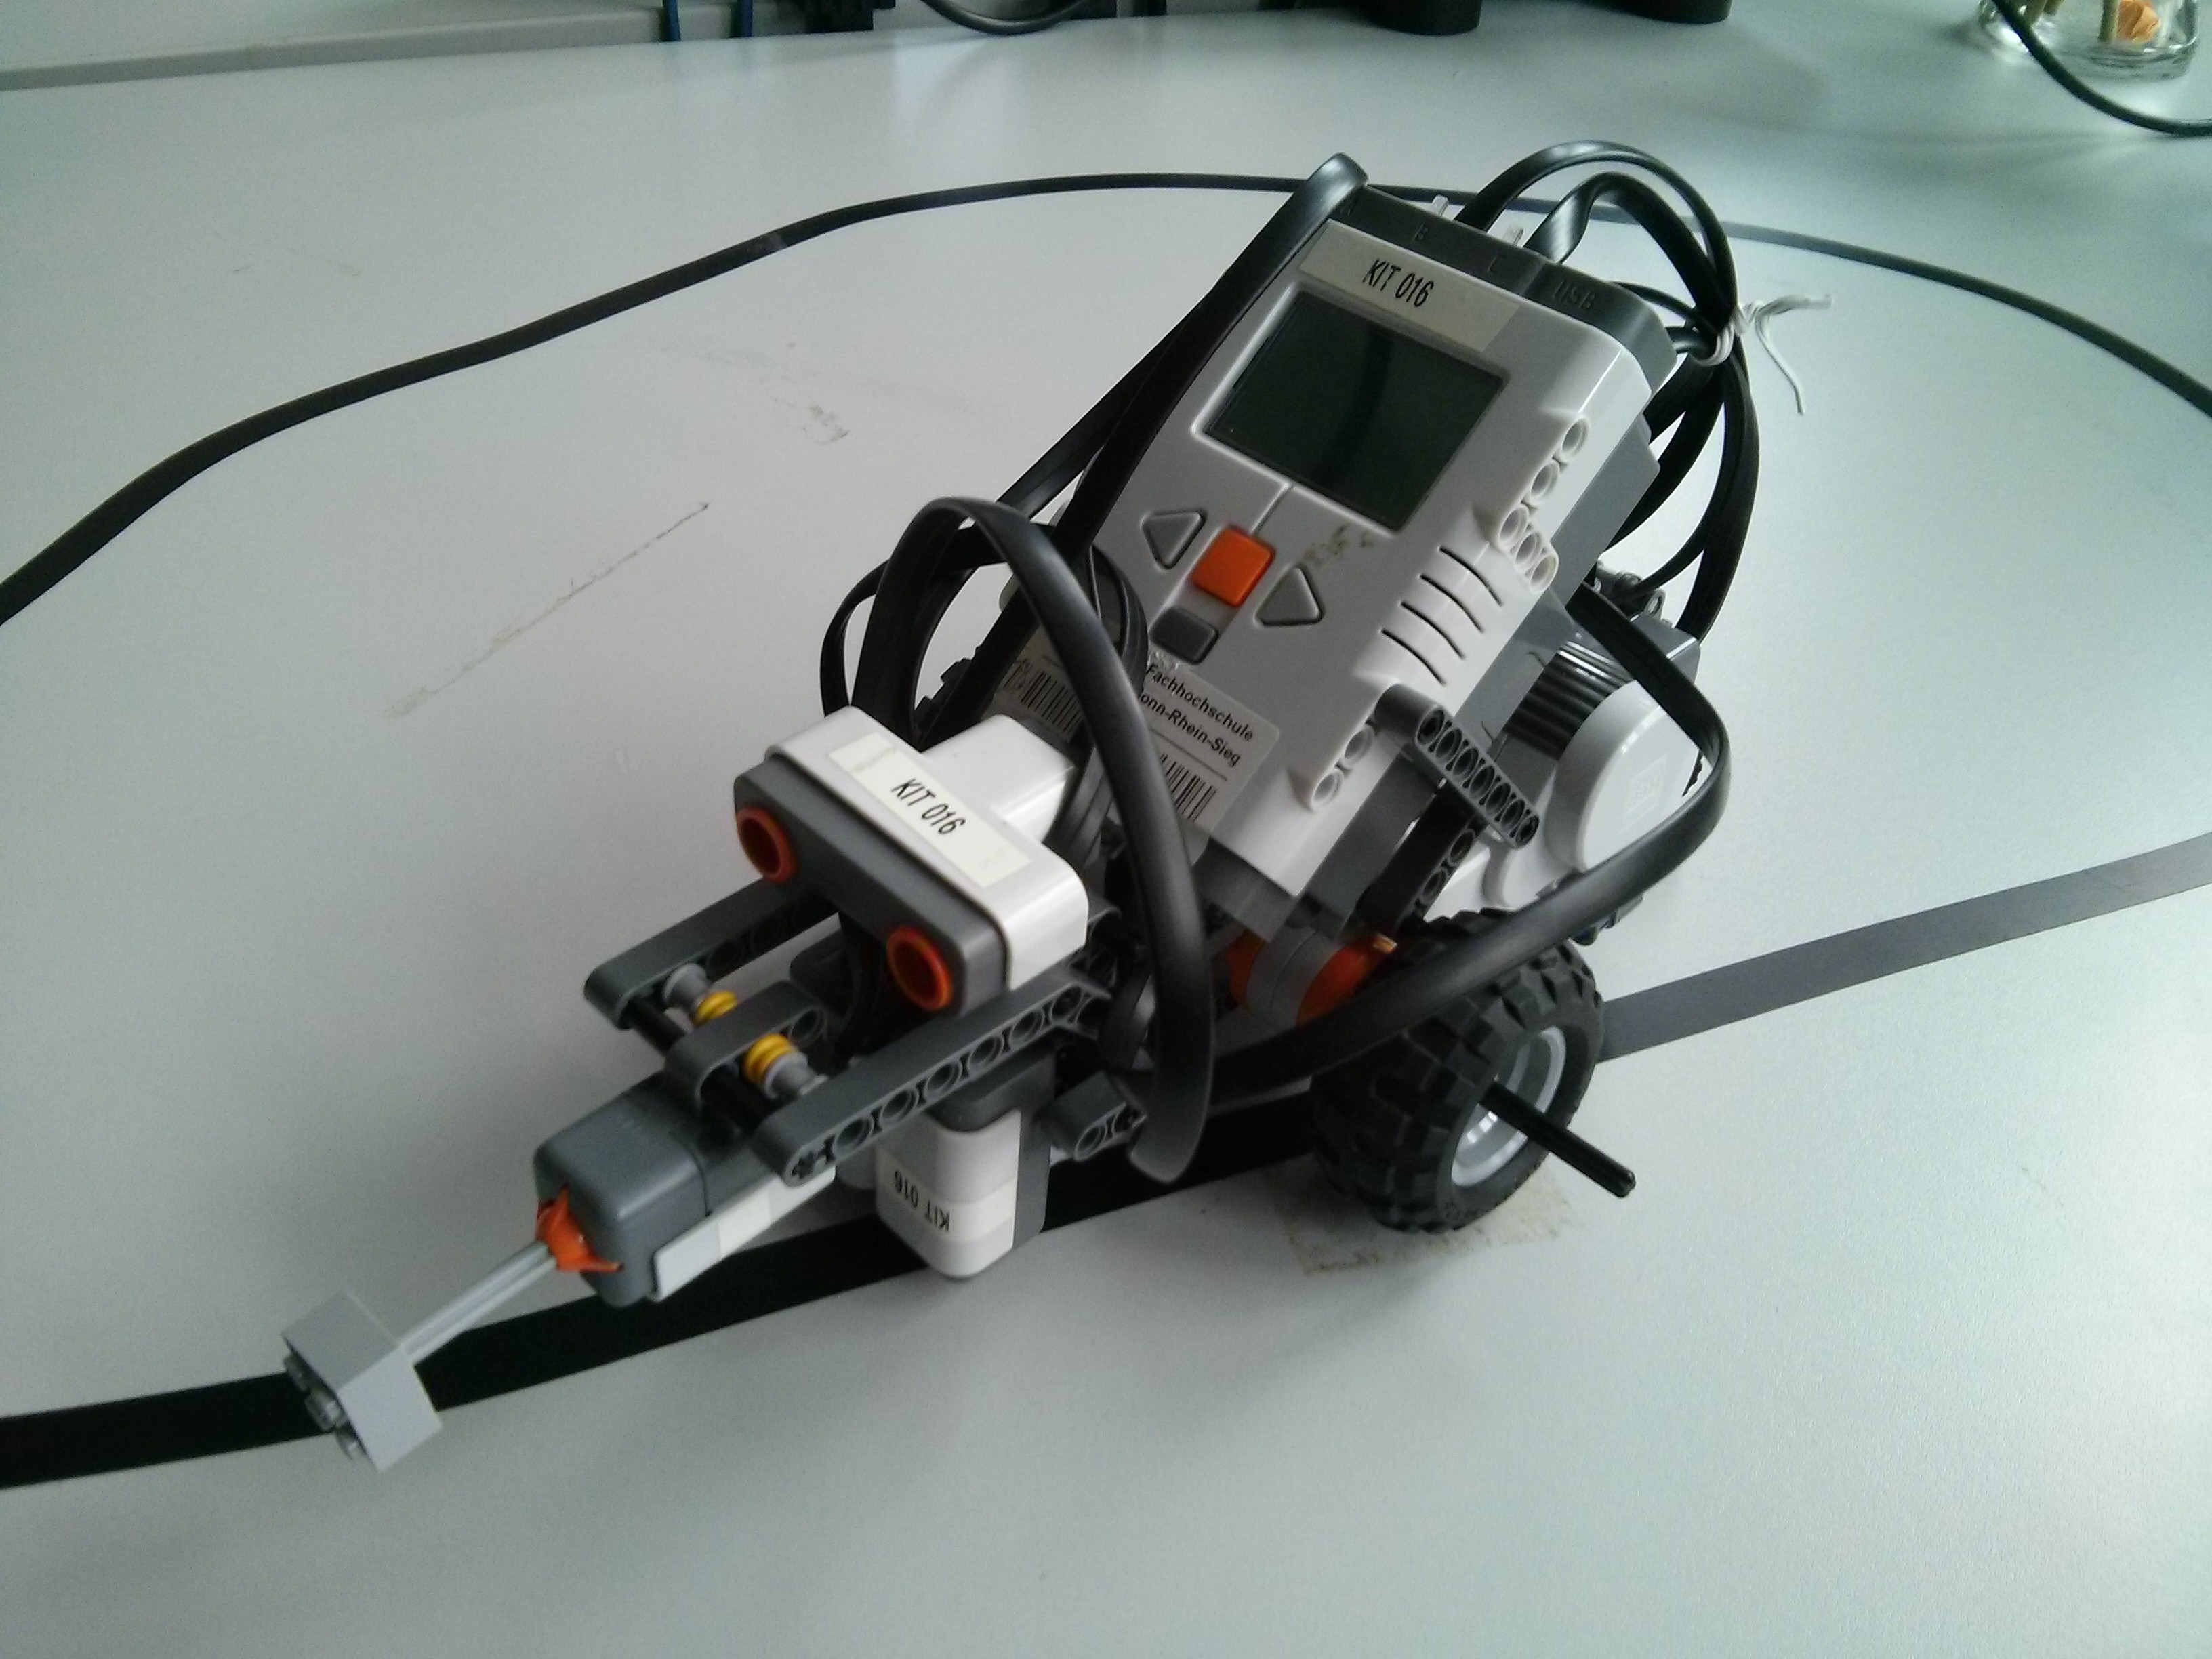
\includegraphics[width=\textwidth, height=\textheight, keepaspectratio]{IMG_20160922_170936.jpg}
	\end{frame}
\end{document}